\section{The RationalGRL Framework}
\label{sect:overview}

In this section we present our RationalGRL framework, which allows stakeholders to discuss, analyse and argue about goal models. The RationalGRL framework includes two main parts: Argumentation and GRL goal modeling. 

The GRL part of RationalGRL allows for the creation of GRL goal models by analyzing the non-functional requirements in the requirements specification document and by refining the high-level goals into operationalized tasks. For the argumentation part, arguments and counterarguments can be put forward about various parts of this goal model.
These two parts, GRL and argumentation, are developed iteratively and each side can impact the other side so that the models can be refined or new critical questions and argument schemes can be instantiated. For example, answering a critical question \emph{Is the task \texttt{A} possible?} can result in removing or adding a task in the GRL model. Similarly,  if, for example, we add a new intentional element to the GRL model, it can lead to a new critical question relevant to this intentional element and its relationships.  

Figure~\ref{fig:rationalgrl-framework} presents an overview of RationalGRL framework. At the bottom there are two activities: \emph{practical reasoning \& argumentation} and \emph{goal model construction}. As already explained, these two activities influence each other: adding elements to a goal model gives rise to new critical questions about these elements, and answering critical questions with arguments may add or delete elements from the GRL model. The activities thus provide two models: a RationalGRL argumentation model (left-hand side), which includes arguments for and against goal model elements, and a GRL goal model (right-hand side). The two types of models are connected by traceability links. In this way, it becomes possible to trace a goal model back to the original argumentative discussion about goals, tasks and requirements.

\begin{figure}[ht]
\centering
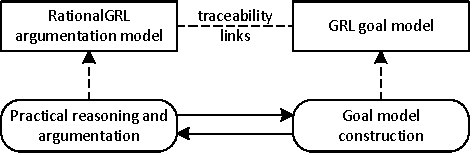
\includegraphics[scale=0.4]{img/framework}
\caption{The RationalGRL Framework\todo{F}{M,S}{Can you make this a vector image?}}
\label{fig:rationalgrl-framework}
\end{figure}

In the rest of this section, we discuss the individual parts of the GRL framework. First we discuss the argument schemes and critical questions that form the basis of our framework (Section~\ref{sect:overview:as}. After this, we explain the RationalGRL language and metamodel (Section~\ref{sect:metamodel}). \todo{F}{all}{finish once paper done}

\subsection{RationalGRL Argument Schemes and Critical Questions}
\label{sect:overview:as}

\begin{table*}[t]
\centering
\begin{tabularx}{\textwidth}{|l|l|l|X|l|l|}
\hline
\multicolumn{2}{|c|}{\textbf{Argument scheme}} & \multicolumn{2}{c|}{\textbf{Critical Questions}} & \textbf{Effect}\\
\hline
AS0 & Actor $a$ is relevant & CQ0 &Is the actor relevant? & DISABLE\\
\hline
AS1 & Actor $a$ has resource $R$ & CQ1 &Is the resource available? & DISABLE\\
\hline
AS2 & Actor $a$ can perform task $T$ & CQ2 &Is the task possible? & DISABLE\\
\hline
AS3 & Actor $a$ has goal $G$ & CQ3 & Can the desired goal be realized? & DISABLE\\
\hline
AS4 & Actor $a$ has softgoal $S$ & CQ4 & Is the softgoal a legitimate softgoal?& DISABLE\\
\hline
\hline
AS5 & Goal $G$ decomposes into tasks $T_1,\ldots,T_n$ & CQ5a & Does the goal decompose into the tasks?& DISABLE\\
& & CQ5b & Does the goal decompose into any other tasks?& REPLACE\\
\hline
AS6 & Task $T$ contributes to softgoal $S$& CQ6a & Does the task contribute to the softgoal?& DISABLE\\
&& CQ6b & Are there alternative ways of contributing to the same softgoal?& INTRO \\
&& CQ6c & Does the task have a side effect which contribute negatively to some other softgoal?& INTRO\\
&& CQ6d & Does the task contribute to some other softgoal?& INTRO\\
\hline
AS7 & Goal $G$ contributes to softgoal $S$ & CQ7a & Does the goal contribute to the softgoal?& DISABLE\\
&& CQ7b & Does the goal contribute to some other softgoal?& INTRO\\
\hline
AS8 & Resource $R$ contributes to task $T$ & CQ8 & Is the resource required in order to perform the task?& DISABLE\\
\hline
AS9 & Actor $a$ depends on actor $b$ & CQ9 & Does the actor depend on any actors?& INTRO\\
\hline
AS10 & Task $T_1$ decomposes into tasks $T_2,\ldots,T_n$ & CQ10a & Does the task decompose into other tasks?& REPLACE\\
 &  & CQ10b & Is the decomposition type correct? (AND/OR/XOR)& REPLACE\\
\hline
AS11 & Task $T$ contributes negatively to softgoal $S$& CQ11 & Does the task contribute negatively to the softgoal?& DISABLE\\
\hline
\hline
AS12 & Element $IE$ is relevant & CQ12 & Is the element relevant/useful? & DISABLE\\
\hline
AS13 & Element $IE$ has name $n$ & CQ13 & Is the name clear/unambiguous? & REPLACE\\
\hline
\hline
- & - & Att & Generic counterargument & ATTACK\\
\hline
\end{tabularx}
\caption{List of argument schemes (AS0-AS13), critical questions (CQ0-CQ12), and the effect of answering them (right column).}
\label{table:argument-schemes}
\end{table*}

A core aspect of the RationalGRL framework are the argument schemes that allow us to talk about the goal models. Recall from section \ref{sect:gmas} that we ended up with a list of argument schemes and critical questions that were found in the transcripts (Table~\ref{table:transcripts:results:argumentschemes}). Using this list as a basis, we further refined our set of argument schemes and critical questions for RationalGRL into the list shown in Table~\ref{table:argument-schemes}. 

The argument schemes AS0-AS4 and AS12-AS13 are arguments for an element of a goal model, and AS5-AS11 are related to links in a goal model. The last scheme (Att) is a scheme for a generic counterargument against any type of argument that has been put forward. 

The critical questions presented in Table~\ref{table:argument-schemes} are related to their respective argument schemes. Answering a critical question in a certain way can have four different effects on the original argument and the corresponding GRL element:

\begin{itemize} 
\item \textsf{INTRO}: Introduce a new goal element or relationship with a corresponding argument. This operation does not attack the original argument to which the question pertains, but rather creates a new argument. In Figure~\ref{fig:transcripts:grl}, each GRL element can be seen as the instantiation of an argument scheme. For instance, the XOR-decomposition from ``Generate Cars'' is an instantiation of AS5 as follows: ``Goal \texttt{Generate cars} XOR-decomposes into tasks \texttt{Keep same cars} and \texttt{Create new cars}''. Suppose now that the modelers that created Figure~\ref{fig:transcripts:grl} would continue their analysis by discussing critical question CQ5b: ``Does the goal \texttt{Generate cars} decompose into other tasks?'', and that they would answer this with ``Yes, namely \texttt{Choose randomly}''. This then results in the introduction of another task with the name ``Choose randomly'', and the XOR-decomposes would go from ``Generate Cars'' into the three tasks \texttt{Keep same cars}, \texttt{Create new cars}, and \texttt{Choose randomly}.'' %SG: Very good example. But should we also show it in the model as a new element?
\item \textsf{DISABLE:} Disable the element or relationship of an argument scheme to which critical questions pertains. This operation does not create a new argument, but it only disables (i.e., attacks) the original one. In Figure~\ref{fig:transcripts:grl}, there are several examples of disabled GRL elements. The task ``Add traffic light'' (top-left in figure) is attacked by answering critical question CQ2: ``Is task Add traffic light possible?'' negatively, resulting in an argument that disables the GRL element. What we also see from Figure~\ref{fig:transcripts:grl} is that actor ``Teacher'' is disabled and thus all the elements that are bound to this actor are disabled as well. Furthermore, disabled task ``Dynamic Simulation'' also disables all incoming and outgoing links with this task.

\item \textsf{REPLACE:} Replace the element of the argument scheme with a new element. In Figure~\ref{fig:transcripts:grl}, task ``Show map editor'' has been replaced various times, and this is shown in the figure as a \emph{refined} element. In this case, participants were discussing the correct naming for this element (CQ13), leading to various replacements of the name. While the previous names are not shown in the figure, they show up in the details pane of the corresponding element. %SG: why generate car has a star but not this one?
\item \textsf{ATTACK:} Attack any argument with an argument that cannot be classified as a critical question. In Figure~\ref{fig:transcripts:grl}, we see one example of such a counter-attack. First, task ``Control car influx per road'' is attack by answering CQ2 (irrelevant task). However, after discussing this, participants found that this was not the case, since the problem description stated that it is important that students can control the simulation manually. Therefore, the argument that attacked the task is attacked by the counter-argument ``Important for students'', which re-enables the task ``Control car influx per road''. We provide a precise semantics for this in Section~\ref{sect:formalframework}.
\end{itemize}

It is important to note that the list of argument schemes and critical questions we present in this section is not exhaustive. It is an initial list that we have obtained by coding transcripts. However, our framework is fully extensible, meaning that new argument schemes and critical questions can be added depending on the problem domain.

\subsection{RationalGRL Metamodel}
\label{sect:metamodel}

Figure~\ref{fig:metamodel} depicts the RationalGRL metamodel linking the main elements of our argumentation extension to the main GRL elements. We describe the metamodel bottom-up, starting with the GRL package.\todo{F}{all}{Fig. 6 is now far removed from where it is mentioned in the text, we should fix this when paper is nearly finished}

The GRL package of our metamodel consists of the core GRL concepts, which constitute a part of the URN metamodel from Recommendation Z.151~\cite{URN}. These concepts represent the abstract grammar of the language, independently of the notation. This metamodel also further defines the GRL concepts and constructs introduced earlier\footnote{Note that for readability, some GRL concepts, such as contribution strength, have been omitted from the figure.}.

The GRL specification consists of \textsf{GRLModelElements}, which can be either \textsf{GRLLinkableElements} or \textsf{ElementLinks}. A \textsf{GRLLinkableElement} can again be specialized into an \textsf{Actor} or an \textsf{IntentionalElement} (which is either a \textsf{Softgoal}, \textsf{Goal}, \textsf{Task}, \textsf{Resource}, or a \textsf{Belief}). Intentional elements can be part of an actor, and \textsf{GRLLinkableElements} are connected through \textsf{ElementLinks} of different types (i.e., \textsf{Contribution, Decomposition}, or \textsf{Dependency}). Note that actors can be connected through links as well, which is done with \textsf{Dependency} links. 

The Argumentation package depicts the concepts we introduced in the previous sections. An \textsf{ArgumentScheme} represents an (uninstantiated) scheme containing variables that can be replaced with intentional elements. \textsf{CriticalQuestions} are possible ways to attack or elaborate an argument scheme. As such, each critical question applies to exactly one scheme, but each scheme can be elaborated or attacked through multiple critical questions. When an argument scheme is instantiated, we obtain an \textsf{Argument}. Therefore, each argument is associated with exactly one scheme, but a scheme can be instantiated in multiple ways. When a critical question is answered, we obtain an \textsf{AttackLink}. Each \textsf{AttackLink} is associated with at most one critical question, but a critical question can be used to attack multiple arguments. Note that an \textsf{AttackLink} can also be associated with no critical questions. This allows the user to create attacks between arguments, which do not necessarily correspond to one of the critical questions. A \textsf{RationalGRLmodel} is composed out of arguments and attack relations.

There is only one link between the \textsf{GRL} package and the \textsf{Argumentation} package, but it is a very important one. The link specifies that each \textsf{GRLModelElement} is in fact an argument. This means that each model element inherits the \textsf{AcceptStatus} as well, allowing GRL elements to be accepted or rejected. This, furthermore, means that argument schemes can be applied to all GRL elements, capturing the intuition that each GRL element can be regarded as an instantiated argument scheme. Note that besides arguments about elements of the GRL model, we also have a \textsf{GenericArgument} which is simply a counter-argument to an existing argument that does not relate to any of the GRL elements, but can come from an external source, for instance a piece of evidence or an expert opinion. We will see various examples of such arguments in the next sections.

\begin{figure*}[h!]
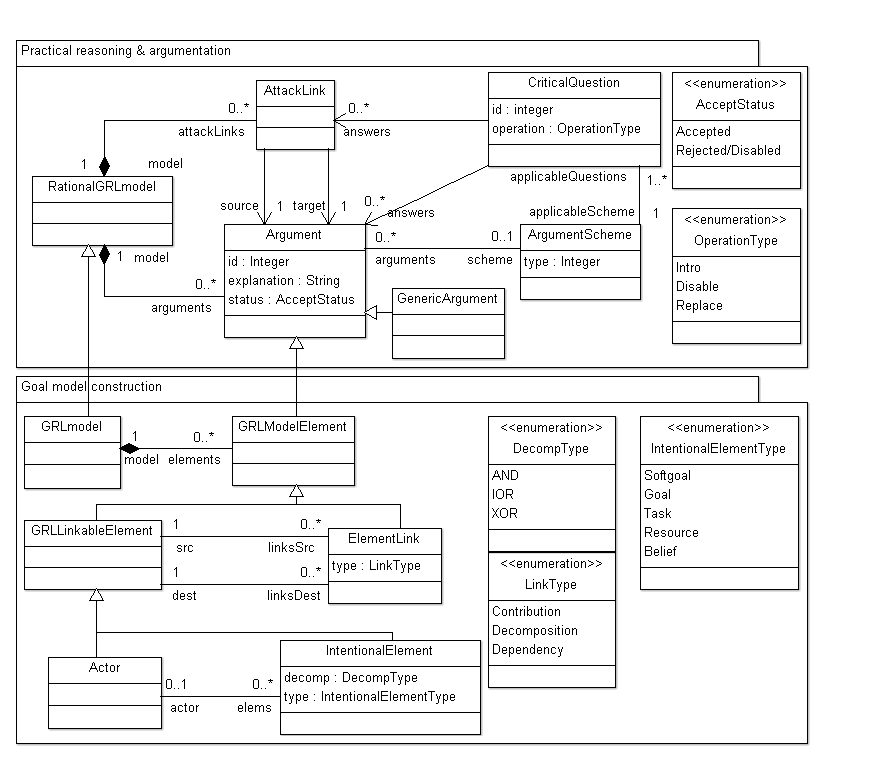
\includegraphics[width=\textwidth]{metamodel/metamodel}
\caption{The RationalGRL metamodel \todo{F}{M}{Change RationalGRLDiagram to RationalGRLmodel}}
\label{fig:metamodel}
\end{figure*}

As an example of a RationalGRL model, consider Figure~\ref{fig:transcripts:grl}, which was created on the basis of transcript $t_1$. This figure shows a simplified version of the actual model in order to improve the presentation, but the full models can be found back in our repository. 

\begin{figure*}[h!]
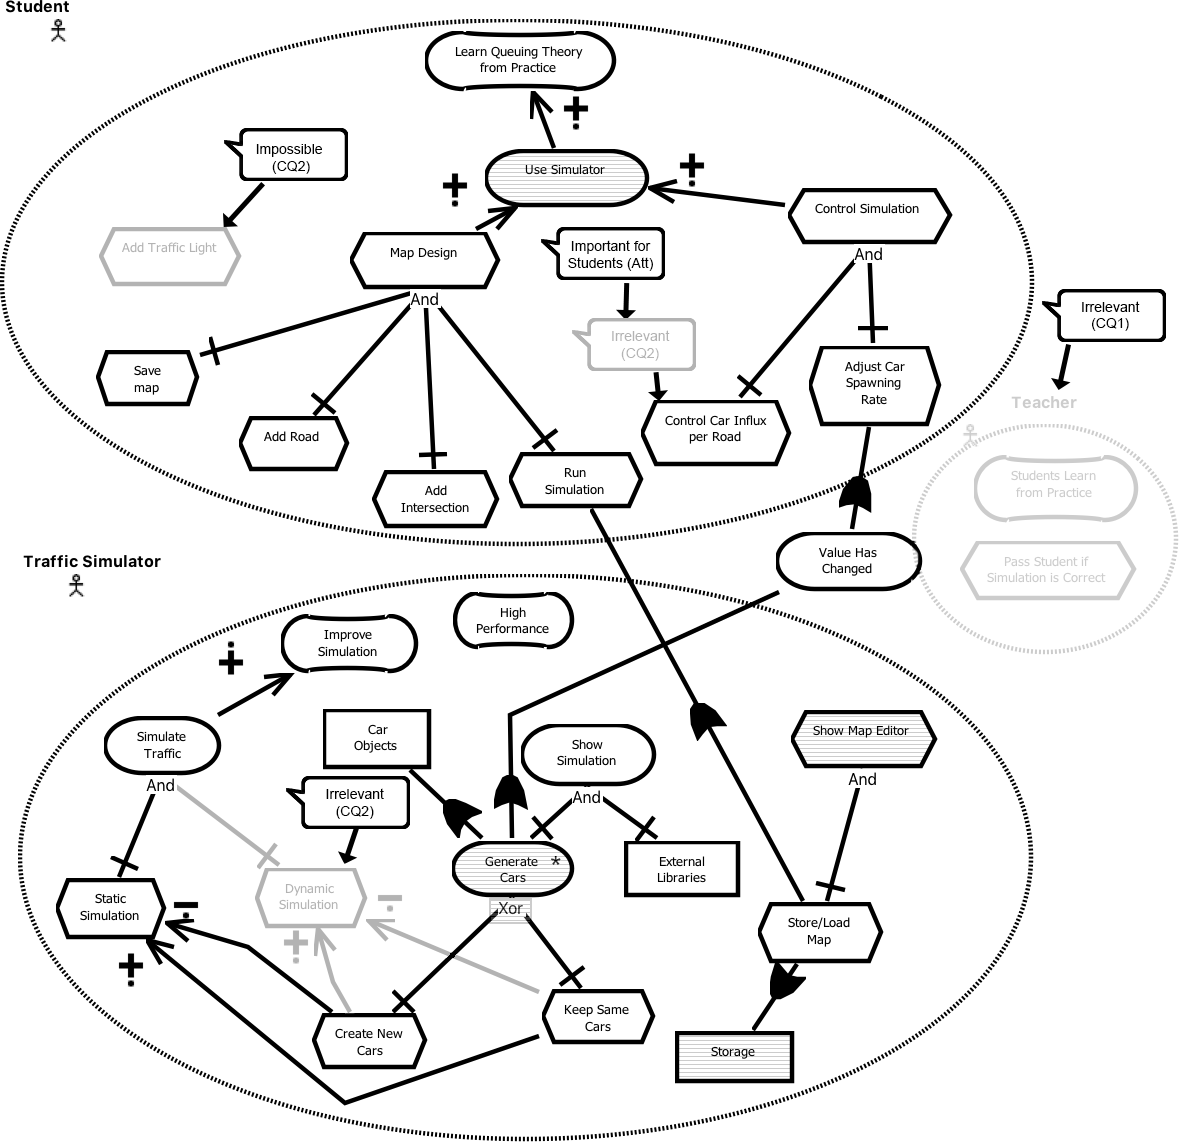
\includegraphics[width=\textwidth]{img/Fig6}
\caption{The GRL model constructed from transcript $t_1$.} 
\label{fig:transcripts:grl}
\end{figure*} 

%I wasn't really sure what to do with the below section. 
\iffalse
\subsection{RationalGRL Language}
The RationalGRL language is an extension of GRL, which means that it includes all the GRL elements shown in Figure~\ref{fig:grl_legend}. However, there are also new elements (Figure~\ref{fig:rationalgrllegend}):

\begin{itemize}
\item \emph{Argument}: This represents an argument that does not correspond to a GRL element. created by answering one of the critical questions which disables a GRL element, or counter-attacks a previous argument. 
\item \emph{Rejected GRL element}: If an argument or GRL element is attacked by an argument, which itself is not attacked, then this GRL element will be rejected, meaning that it does not play a role in the analysis of the GRL model. The status of arguments and 
\item \emph{Refined GRL Element}: Not all critical questions attack a GRL element. It is also possible that a critical question \emph{replaces} an existing element (for instance, by clarifying the name of the element), or that it leads to the \emph{introduction} of a new element. In these cases, the corresponding GRL element is shown with a striped background. \todo{F}{S,M}{Disabled and Refined GRL elements are not in the metamodel}
\item \emph{Attack Link}: An attack link can occur between an argument and a GRL element, or between two elements. It means that the source argument or element attacks the target argument or element.
\end{itemize} 

\begin{figure}[h]
\centering
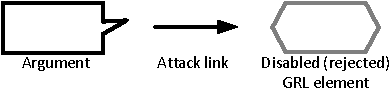
\includegraphics[width=0.35\textwidth]{img/legend}
\caption{The new elements and link of RationalGRL}
\label{fig:rationalgrllegend}
\end{figure}
\fi

\subsection{RationalGRL Methodology} 

We propose the following methodology (shown in Figure~\ref{fig:rationalgrl-methodology}) to develop an instance of the RationalGRL framework. Here we assume that the initial GRL models have been created based on the requirements specification documents and the discussions of the stakeholders. The rest of the steps are as follows:

\begin{figure*}[ht]
\centering

\includegraphics[scale=0.4]{img/methodology}
\caption{The RationalGRL Methodology\todo{F}{M,S}{Can you make this a vector image?}}
\label{fig:rationalgrl-methodology}
\end{figure*}


\textbf{(1) Instantiate Argument Schemes (AS)} -- In this step, we start from the list of arguments schemes of the argumentation framework. We select an intentional element from the initial GRL model that we want to analyze and we instantiate a relevant argument scheme from the already existing list of argument schemes or by adding a new one. For example, an argument scheme can be "Goal \emph{G} contributes to softgoal \emph{S}". When an argument scheme is instantiated, it corresponds to  an argument for or against part of a goal model.

\textbf{(2) Answer Critical Questions (CQs)} -- After instantiating an argument scheme, we invoke related critical questions to attack the argument with counter-arguments.  Each argument scheme includes one or more critical questions. For example, for the argument scheme, "Goal \emph{G} contributes to softgoal \emph{S}", there are two critical questions as follows:  \emph{Does the goal contribute to the softgoal?} and \emph{Does the goal contribute to some other softgoals?}. 
%It is worth mentioning that, answering a critical question may result in a "conflict" situation. This is out of the scope of our work here.  
%MvZ: removed this sentence because I don't know what you mean with "conflict". I think We should explain it better or leave it out.
When the analyst answers  a critical question, a new argument scheme may be instantiated.  Thus, it is possible to go back and forth between this step and step (1).

\textbf{(3) Decide on Intentional Elements and their Relationships} -- By answering a critical question, one of the four following cases can occur: \textsf{INTRO}, \textsf{DISABLE}, \textsf{REPLACE} or \textsf{ATTACK}.  Any of these cases can  impact the arguments and corresponding GRL intentional elements.  \textsf{INTRO} means that 
a new argument scheme is created. That means, the current argument scheme related to the critical question does not get attacked.  In the case of \textsf{DISABLE}, the intentional element or its related links are disabled or removed from the models. \textsf{REPLACE} introduces a new argument and attacks the original argument at the same time. This means that the original element of the argument scheme is replaced with a new one. \textsf{ATTACK} is a generic counterargument which attacks any argument with another argument when new evidence occurs.  

\textbf{(4) Modify GRL Models} -- In this step, we modify the GRL models based on the situation of step (3). That is, one of the following situation can happen with respect to the initial GRL model: 1) a new intentional element or a new link is introduced; 2) an existing intentional element or an existing link gets disabled (removed) from the model; or 3) an existing intentional element or link is replaced by a new one. This results in a new modified GRL. The new GRL model can then impact the argument schemes and instantiate another argument scheme (Step (1)).   

We can continue these four steps until there is no more intentional element or link to analyze or we reach a satisfactory model. 